% Tutorial TCC for the abntexto-ufc class.
% Edit the metadata below, then replace the example academic content.

\DocumentMetadata{
  lang = pt-BR,
  pdfstandard = A-2b,
  pdfversion = 1.7
}

\documentclass{abntexto-ufc}

% Main document configuration.
% Required fields depend on the selected document profile.
\ufcsetup{
  type = undergraduate-capstone,
  print-mode = single-sided,
  cover = auto,
  catalog-card = false,
  coat-of-arms = true,
  % Typography and optional modules.
  font = times,
  strict-font = false,
  tables = tabularray,
  code = listings,
  algorithms = none,
  glossary = glossaries,
  index = none,
  % Institution and course.
  institution = {Universidade Federal do Ceará},
  center = {Nome do Centro, Faculdade, Instituto ou Campus},
  department = {},
  undergraduate-program = {Ciência da Computação},
  undergraduate-degree = {bacharel},
  % Author and work.
  author = {Nome Completo do Autor},
  title = {Validação automatizada de documentos acadêmicos em LaTeX},
  subtitle = {um estudo demonstrativo},
  location = {Fortaleza},
  year = {2026},
  % Approval data.
  approval-date = {12 de setembro de 2026},
  advisor = {Prof. Dr. Nome do Orientador},
  advisor-institution = {Universidade Federal do Ceará (UFC)},
  examiner-2 = {Profa. Dra. Nome do Segundo Membro},
  examiner-2-institution = {Universidade Federal do Ceará (UFC)},
  examiner-3 = {Prof. Dr. Nome do Terceiro Membro},
  examiner-3-institution = {Universidade Federal do Ceará (UFC)}
}

% Bibliography and glossary sources.
\ufcAddBibliographyResource{backmatter/references.bib}
\newglossaryentry{normalizacao}{
  name = {normalização},
  description = {aplicação sistemática das normas e orientações pertinentes à apresentação do trabalho acadêmico}
}

\newglossaryentry{validacao}{
  name = {validação},
  description = {processo de observar critérios definidos e registrar se o artefato avaliado atende às condições verificadas}
}


\begin{document}

% ----------------------------------------------------------------------
% Front matter
% ----------------------------------------------------------------------
\pretextual

\ufcPrintCover
\ufcPrintTitlePage
\ufcPrintApprovalPage

% Optional front-matter elements.
% Uncomment only what is applicable to the real work.
% \ufcPrintCatalogCard{frontmatter/catalog-card}
% \ufcPrintErrata{frontmatter/errata}
% \ufcPrintDedication{frontmatter/dedication}
% \ufcPrintAcknowledgments{frontmatter/acknowledgments}
% \ufcPrintEpigraph{frontmatter/epigraph}

\ufcPrintSummary{frontmatter/summary}
\ufcPrintAbstract{frontmatter/abstract}

% Keep only the lists that are useful for the final document.
\ufcPrintListOfIllustrations
\ufcPrintListOfTables
\ufcPrintListOfCodeListings
\ufcPrintTableOfContents

% ----------------------------------------------------------------------
% Main matter
% ----------------------------------------------------------------------
\textual

\section{Introdução}\label{sec:introduction}

A preparação de um trabalho acadêmico envolve duas responsabilidades distintas: produzir conteúdo científico consistente e apresentar esse conteúdo de acordo com as regras aplicáveis. Em documentos extensos, ajustes manuais de margens, títulos, listas, citações e elementos pré-textuais aumentam o risco de inconsistência e dificultam a repetição do processo. Sistemas de preparação de documentos como o \LaTeX{} permitem separar conteúdo e apresentação e automatizar parte desse trabalho \parencite{lamport1994}.

Na Universidade Federal do Ceará (UFC), a normalização acadêmica combina normas técnicas vigentes e orientações institucionais publicadas pelo Sistema de Bibliotecas \parencite{ufc2026normalizacao}. Nesse contexto, uma classe documental pode reduzir tarefas repetitivas, mas não elimina a necessidade de revisar o texto, conferir as fontes consultadas e verificar os requisitos específicos do curso ou programa.

Este TCC é um exemplo didático. O tema escolhido permite mostrar, em um documento curto, como organizar um trabalho real e como usar os principais recursos do \texttt{abntexto-ufc}. Explicações detalhadas da API permanecem na documentação do projeto; o corpo deste trabalho segue a estrutura acadêmica usual.

\subsection{Problema}

Mesmo quando um modelo automatiza a apresentação, erros podem surgir por configuração inadequada, conteúdo incompleto ou diferenças entre o fonte e o PDF final. O problema considerado neste estudo é como organizar um fluxo simples capaz de compilar e verificar automaticamente propriedades básicas de um documento acadêmico antes da revisão humana.

\subsection{Objetivos}

O objetivo geral é descrever um fluxo demonstrativo de validação automatizada de documentos acadêmicos produzidos em \LaTeX{}.

Como objetivos específicos, pretende-se:

\begin{ufclettereditems}
  \item organizar o documento em etapas reprodutíveis de preparação, compilação e verificação;
  \item observar propriedades do PDF que podem ser verificadas automaticamente;
  \item registrar resultados de uma execução sintética do fluxo;
  \item destacar quais decisões continuam dependentes de revisão humana.
\end{ufclettereditems}

\subsection{Organização do trabalho}

Além desta introdução, a Seção~\ref{sec:background} apresenta os conceitos necessários; a Seção~\ref{sec:methodology} descreve o procedimento demonstrativo; a Seção~\ref{sec:results} reúne os resultados sintéticos; e a Seção~\ref{sec:conclusion} apresenta as considerações finais.

\section{Fundamentação teórica}\label{sec:background}

\subsection{Preparação de documentos em LaTeX}

O \LaTeX{} trabalha com arquivos fonte que descrevem a estrutura e o conteúdo do documento. A apresentação é obtida durante a compilação, o que favorece o reaproveitamento de estilos e a separação entre a escrita acadêmica e decisões tipográficas repetitivas \parencite{lamport1994}. Essa característica é especialmente útil em trabalhos longos, nos quais referências cruzadas, sumário e bibliografia precisam permanecer coerentes após sucessivas alterações.

Neste tutorial, cada capítulo é mantido em um arquivo próprio. O arquivo \texttt{main.tex} concentra apenas configuração, ordem dos elementos e chamadas principais. Essa divisão torna mais simples localizar o conteúdo que o estudante realmente precisa editar.

\subsection{Normalização acadêmica}

A apresentação de trabalhos acadêmicos é orientada por normas técnicas e, no contexto institucional, por regras complementares. A NBR 14724 estabelece a estrutura geral dos trabalhos acadêmicos \parencite{abnt14724}; citações são tratadas pela NBR 10520 \parencite{abnt10520}; e a elaboração das referências segue a NBR 6023 vigente \parencite{abnt6023}.

A \gls{normalizacao} não deve ser entendida como substituta da qualidade científica. Seu papel é tornar a apresentação previsível, legível e verificável. Por isso, este exemplo usa a classe para concentrar a formatação e reserva ao autor a responsabilidade sobre argumentos, fontes e resultados.

\subsection{Citações e referências}

As referências bibliográficas são armazenadas em \texttt{backmatter/references.bib}. Quando a autoria participa da frase, pode-se escrever, por exemplo, que \textcite{lamport1994} apresenta o sistema \LaTeX{} como uma ferramenta de preparação documental. Quando a fonte aparece apenas como apoio à afirmação, usa-se a forma parentética \parencite{abnt6023}.

O uso de comandos bibliográficos evita digitar manualmente autor e ano e facilita a manutenção da lista final. Citações diretas, quando necessárias em um trabalho real, devem reproduzir fielmente a fonte consultada e incluir o localizador aplicável.

\subsection{Validação reprodutível}

Neste estudo, \gls{validacao} significa observar propriedades mensuráveis do arquivo produzido e registrar o resultado de forma repetível. Nem todo requisito acadêmico pode ser reduzido a um teste automático. Clareza do texto, adequação metodológica, pertinência das conclusões e qualidade das fontes continuam dependendo de avaliação intelectual e revisão humana.

\section{Metodologia}\label{sec:methodology}

O estudo demonstrativo organiza o fluxo em quatro etapas: preparar os arquivos fonte, compilar o documento, executar verificações automáticas e revisar visualmente o PDF. A Figura~\ref{fig:validation-flow} resume essa sequência.

% Object example: identify the figure, declare the source, then render it.
\legend{figure}{Fluxo simplificado da validação automatizada}
\ufcSource{Elaboração própria.}
\label{fig:validation-flow}
\begin{ufcobject}[here]
  \centering
  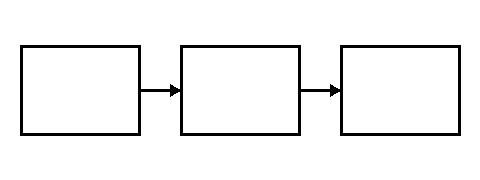
\includegraphics[width=0.65\linewidth]{figures/example-flow.png}
\end{ufcobject}

\subsection{Etapas do procedimento}

O procedimento foi organizado da seguinte forma:

\begin{enumerate}
  \item preencher os metadados e o conteúdo do documento;
  \item compilar o projeto pelo fluxo completo;
  \item verificar propriedades objetivas do PDF;
  \item inspecionar visualmente o resultado antes da entrega.
\end{enumerate}

A Tabela~\ref{tab:checks} apresenta um conjunto mínimo de verificações automáticas usado apenas como exemplo metodológico.

% Numerical table example using the tabularray module.
\begin{table}[htbp]
\centering
\begin{tallabnttblr}
[
  caption={Critérios observados no procedimento demonstrativo},
  label={tab:checks},
  remark{Fonte}={Elaboração própria.},
]
{
  colspec={X[l] X[c] X[l]},
}
\toprule
Critério & Saída & Finalidade \\
\midrule
Tamanho da página & PASS/FAIL & Confirmar o formato A4 \\
Fontes incorporadas & PASS/FAIL & Reduzir dependências externas no PDF \\
PDF/A & PASS/FAIL & Verificar o alvo arquivístico adotado \\
Marcadores estruturais & PASS/FAIL & Confirmar elementos esperados \\
\bottomrule
\end{tallabnttblr}
\end{table}

\subsection{Métrica sintética}

Para resumir uma execução didática, define-se a taxa de verificações aprovadas pela Equação~\ref{eq:pass-rate}, em que $p$ representa o número de verificações aprovadas e $n$ o total executado.

\begin{equation}
  R = \frac{p}{n}\times 100
  \label{eq:pass-rate}
\end{equation}

A métrica não representa qualidade acadêmica. Ela apenas resume o subconjunto de verificações automatizadas escolhido para o exemplo.

\subsection{Exemplo de código}

O Código~\ref{code:mean-score} mostra como incluir um arquivo externo no documento. O conteúdo é propositalmente pequeno para que o foco permaneça na estrutura do TCC.

% Code example: configure the language, identify the object and include the file.
\legend{code}{Função auxiliar para cálculo da média}
\ufcSource{Elaboração própria.}
\label{code:mean-score}
\begin{ufcobject}[here]
  \ufcInputListing[language=Python]{figures/example.py}
\end{ufcobject}

O mesmo mecanismo pode ser usado para trechos maiores, desde que o código seja relevante para o trabalho e permaneça legível no PDF.

\section{Resultados e discussão}\label{sec:results}

A execução sintética considerou quatro verificações automáticas. Todas foram marcadas como aprovadas para demonstrar a forma de registro de resultados; esses valores não correspondem a um experimento científico externo e não devem ser reutilizados como evidência em outro trabalho.

\begin{table}[htbp]
\centering
\begin{tallabnttblr}
[
  caption={Resultados sintéticos da validação},
  label={tab:results},
  remark{Fonte}={Elaboração própria.},
  remark{Nota}={Dados exclusivamente demonstrativos.},
]
{
  colspec={X[l] X[c]},
}
\toprule
Verificação & Resultado \\
\midrule
Formato A4 & PASS \\
Fontes incorporadas & PASS \\
PDF/A & PASS \\
Marcadores estruturais & PASS \\
\bottomrule
\end{tallabnttblr}
\end{table}

Com $p=4$ e $n=4$, a Equação~\ref{eq:pass-rate} produz $R=100\%$. Esse valor deve ser interpretado apenas dentro do cenário construído. Um fluxo de validação real pode incluir dezenas de verificações, resultados de revisão e condições específicas do perfil documental.

\subsection{Interpretação}

Os resultados ilustram duas vantagens da automação. A primeira é a possibilidade de detectar problemas repetitivos antes da revisão final. A segunda é registrar o mesmo procedimento em execuções futuras, reduzindo a dependência de conferências manuais para propriedades objetivas.

Por outro lado, um conjunto de testes aprovado não prova que o texto está academicamente correto. Um PDF pode apresentar dimensões, fontes e referências tecnicamente válidas e ainda conter problemas de argumentação, metodologia ou interpretação. Assim, a automação deve complementar, e não substituir, a revisão do autor, do orientador e das instâncias institucionais aplicáveis.

\subsection{Uso do modelo}

No contexto deste TCC tutorial, o principal resultado é a própria organização do projeto: configuração concentrada no arquivo principal, capítulos separados, bibliografia estruturada e objetos acadêmicos inseridos onde são efetivamente discutidos. Essa organização permite que o estudante substitua o conteúdo demonstrativo pelo seu trabalho sem precisar conservar páginas de documentação dentro do PDF final.

\section{Conclusão}\label{sec:conclusion}

Este trabalho apresentou um fluxo demonstrativo para validação automatizada de documentos acadêmicos produzidos em \LaTeX{}. A proposta separou preparação, compilação, verificações automáticas e revisão visual, mostrando como propriedades objetivas do PDF podem ser verificadas sem atribuir à automação decisões que continuam dependentes de análise humana.

O exemplo também demonstrou uma forma de organizar o projeto acadêmico: o arquivo principal concentra metadados e ordem dos elementos, enquanto capítulos, resumo, abstract, referências e materiais complementares permanecem em arquivos específicos. Figuras, tabelas, equações e código aparecem no contexto metodológico em que são utilizados.

Como limitação, os resultados apresentados são sintéticos e servem apenas para mostrar a estrutura do documento. Em um TCC real, objetivos, método, dados, resultados e conclusões devem decorrer da pesquisa efetivamente realizada. A documentação completa dos comandos da classe permanece separada deste texto para que o PDF do aluno continue sendo um trabalho acadêmico, e não um manual do template.


% ----------------------------------------------------------------------
% Back matter
% ----------------------------------------------------------------------
\ufcPrintReferences
\ufcPrintGlossary

% Material written by the author.
\appendix{Checklist de validação usado no estudo demonstrativo}
\label{ap:validation-checklist}

Este apêndice exemplifica material elaborado pelo próprio autor. No estudo demonstrativo, o checklist mínimo utilizado foi:

\begin{enumerate}
  \item confirmar que o documento foi compilado sem erros;
  \item verificar o tamanho A4 das páginas;
  \item verificar a incorporação das fontes utilizadas;
  \item executar a validação PDF/A disponível no ambiente;
  \item confirmar a presença dos principais elementos estruturais;
  \item revisar visualmente o PDF completo.
\end{enumerate}

Em um trabalho real, substitua este conteúdo por material autoral complementar que seja pertinente à pesquisa.


% External material or material not written by the author.
\annex{Documento complementar externo}
\label{an:external-document}

Este anexo demonstra a posição reservada para um documento complementar que não tenha sido elaborado pelo autor do trabalho.

Substitua este texto pelo material externo efetivamente necessário à pesquisa. Verifique previamente direitos de uso, legibilidade e compatibilidade com o arquivo final.

\noindent\textbf{Fonte:} Instituição ou autor responsável pelo documento externo (ano). Substitua esta indicação pela fonte real do material anexado.


% Optional index:
% set index=imakeidx, mark terms with \index{...}, then uncomment:
% \ufcPrintIndex

\end{document}
